% Tabelle e figure tolte dalla sezione Analisi Dati della relazione.

\begin{figure}[htbp]
    \centering
     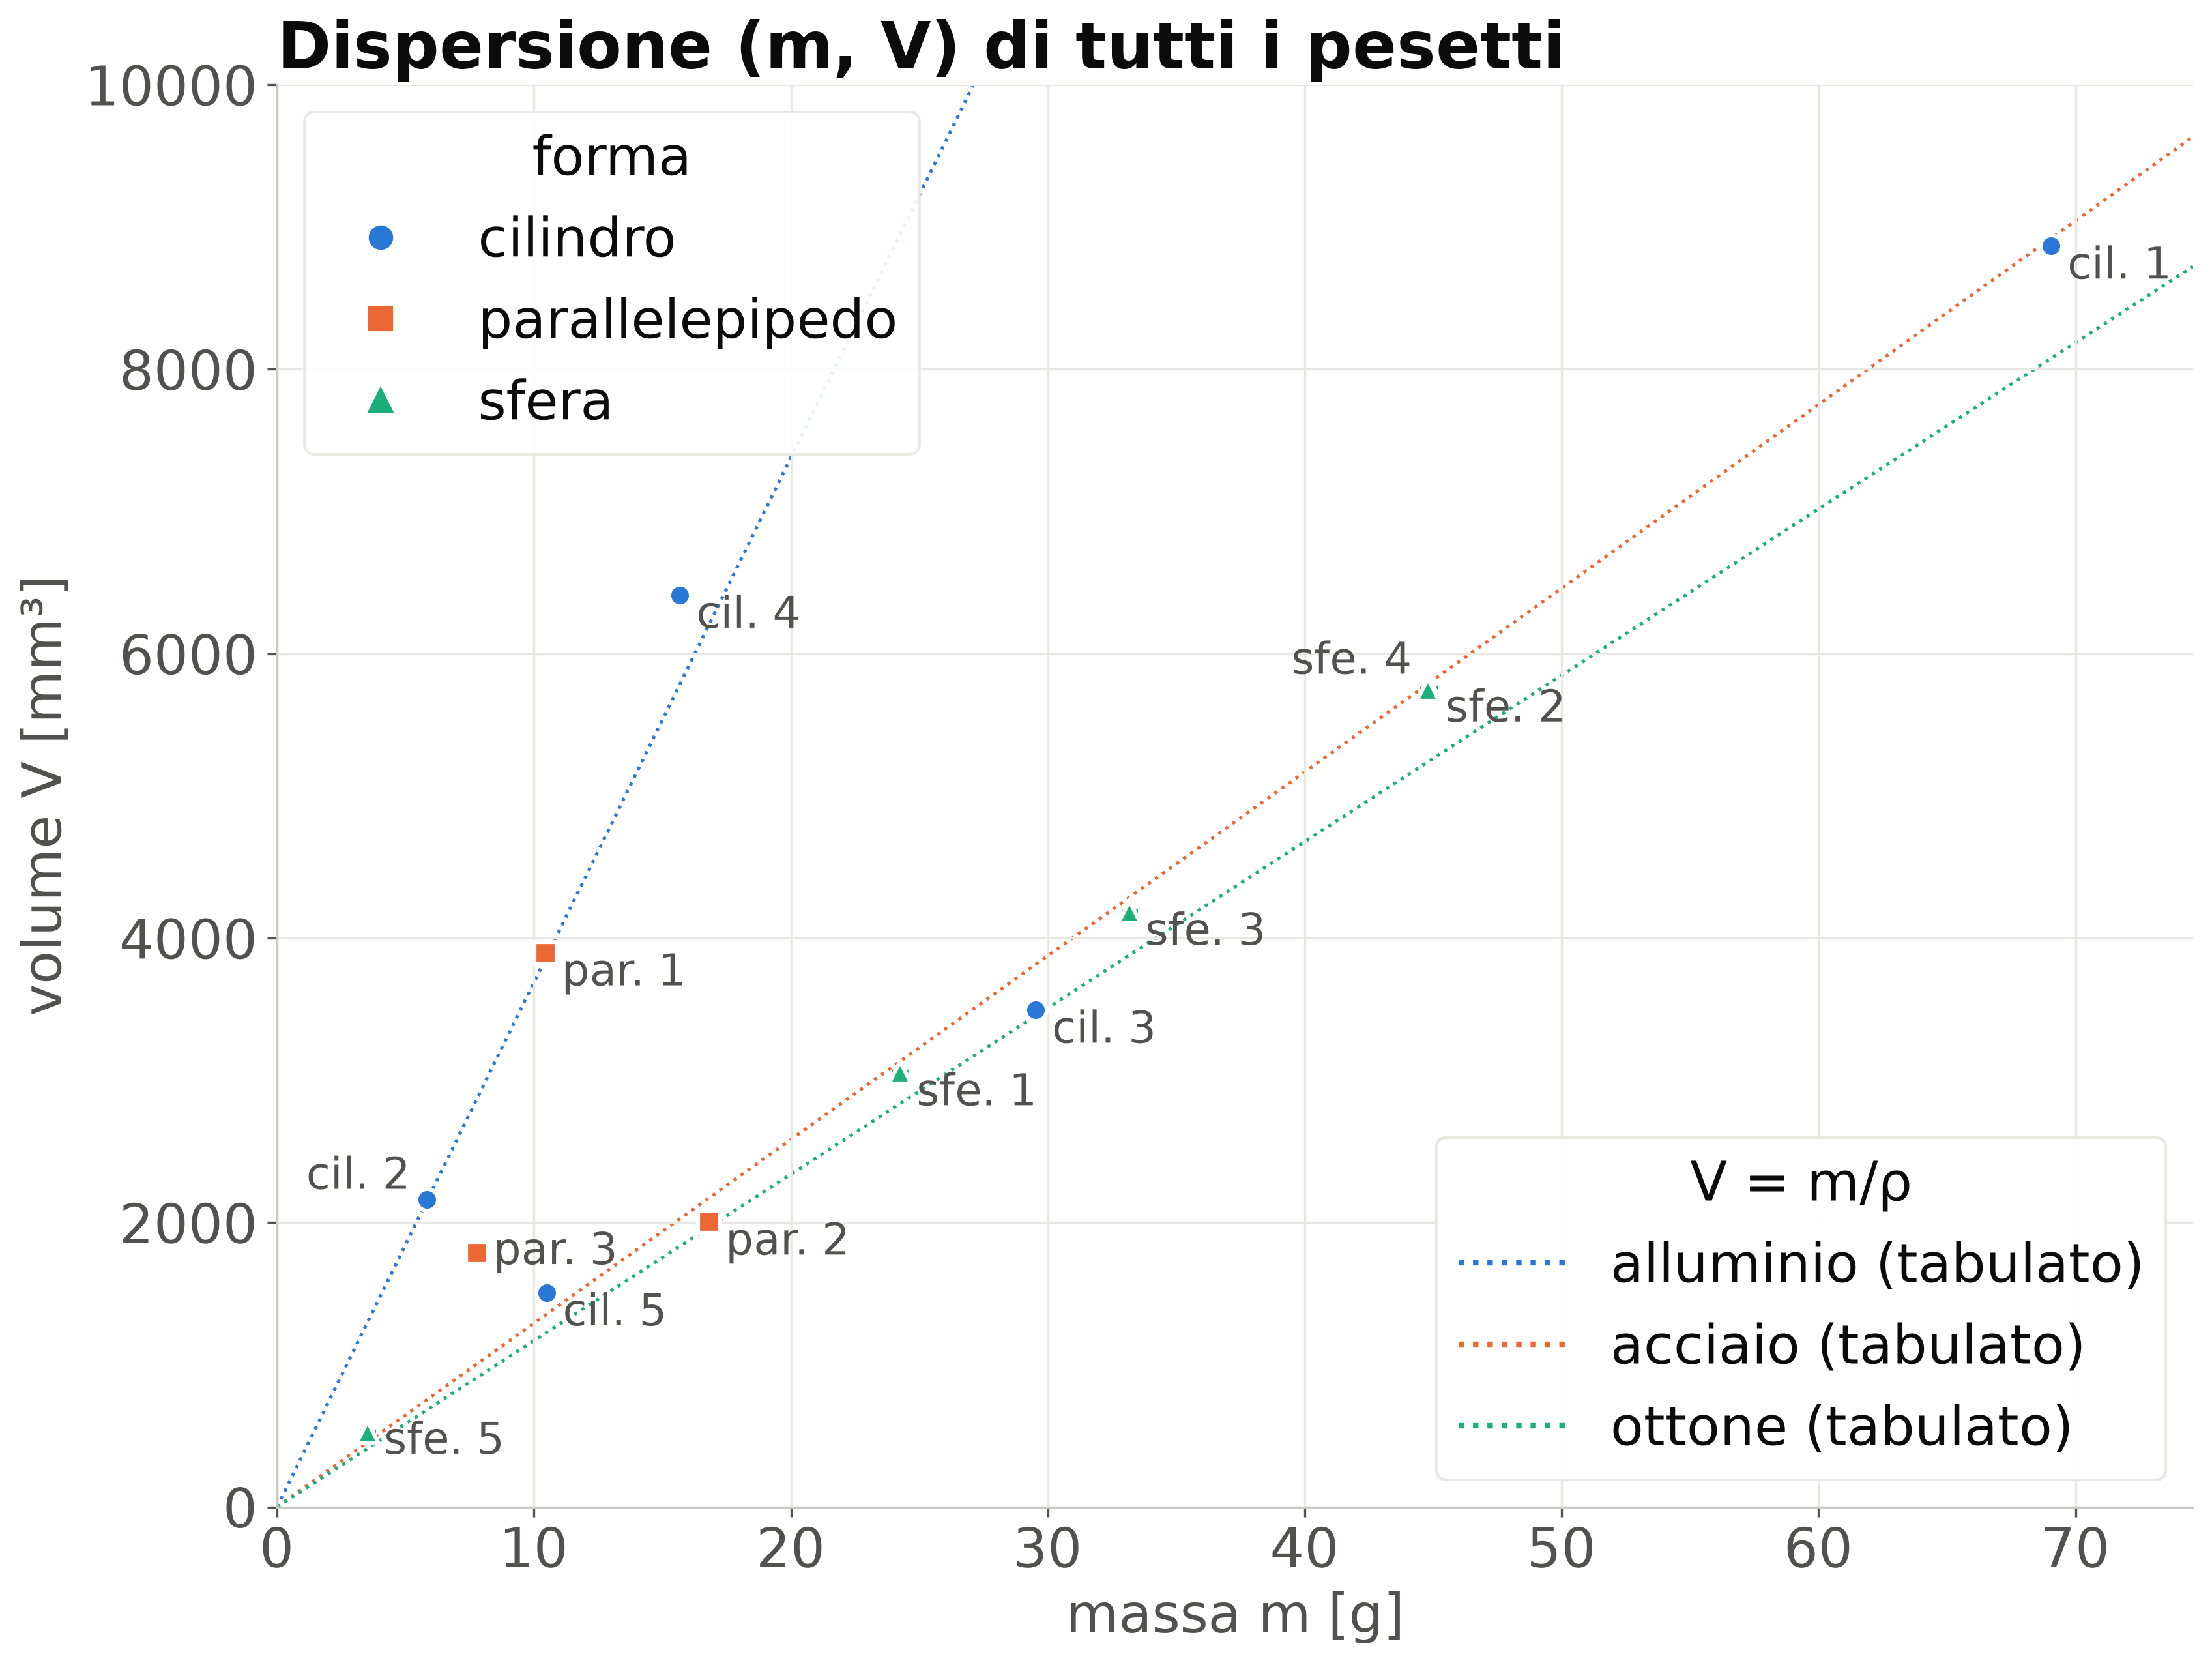
\includegraphics[width=0.75\linewidth]{grafici/a_dispersione_massa_volume.png}
    \caption{Grafico di dispersione $(m,V)$ di tutti i pesetti. Le rette tratteggiate sono $V = m/\rho$ con le densit\`a tabulate di alluminio, acciaio (centro dell'intervallo) e ottone; le barre d'errore sono pi\`u piccole dei punti.}
    \label{fig:dispersione}
\end{figure}

\begin{figure}[htbp]
    \centering
     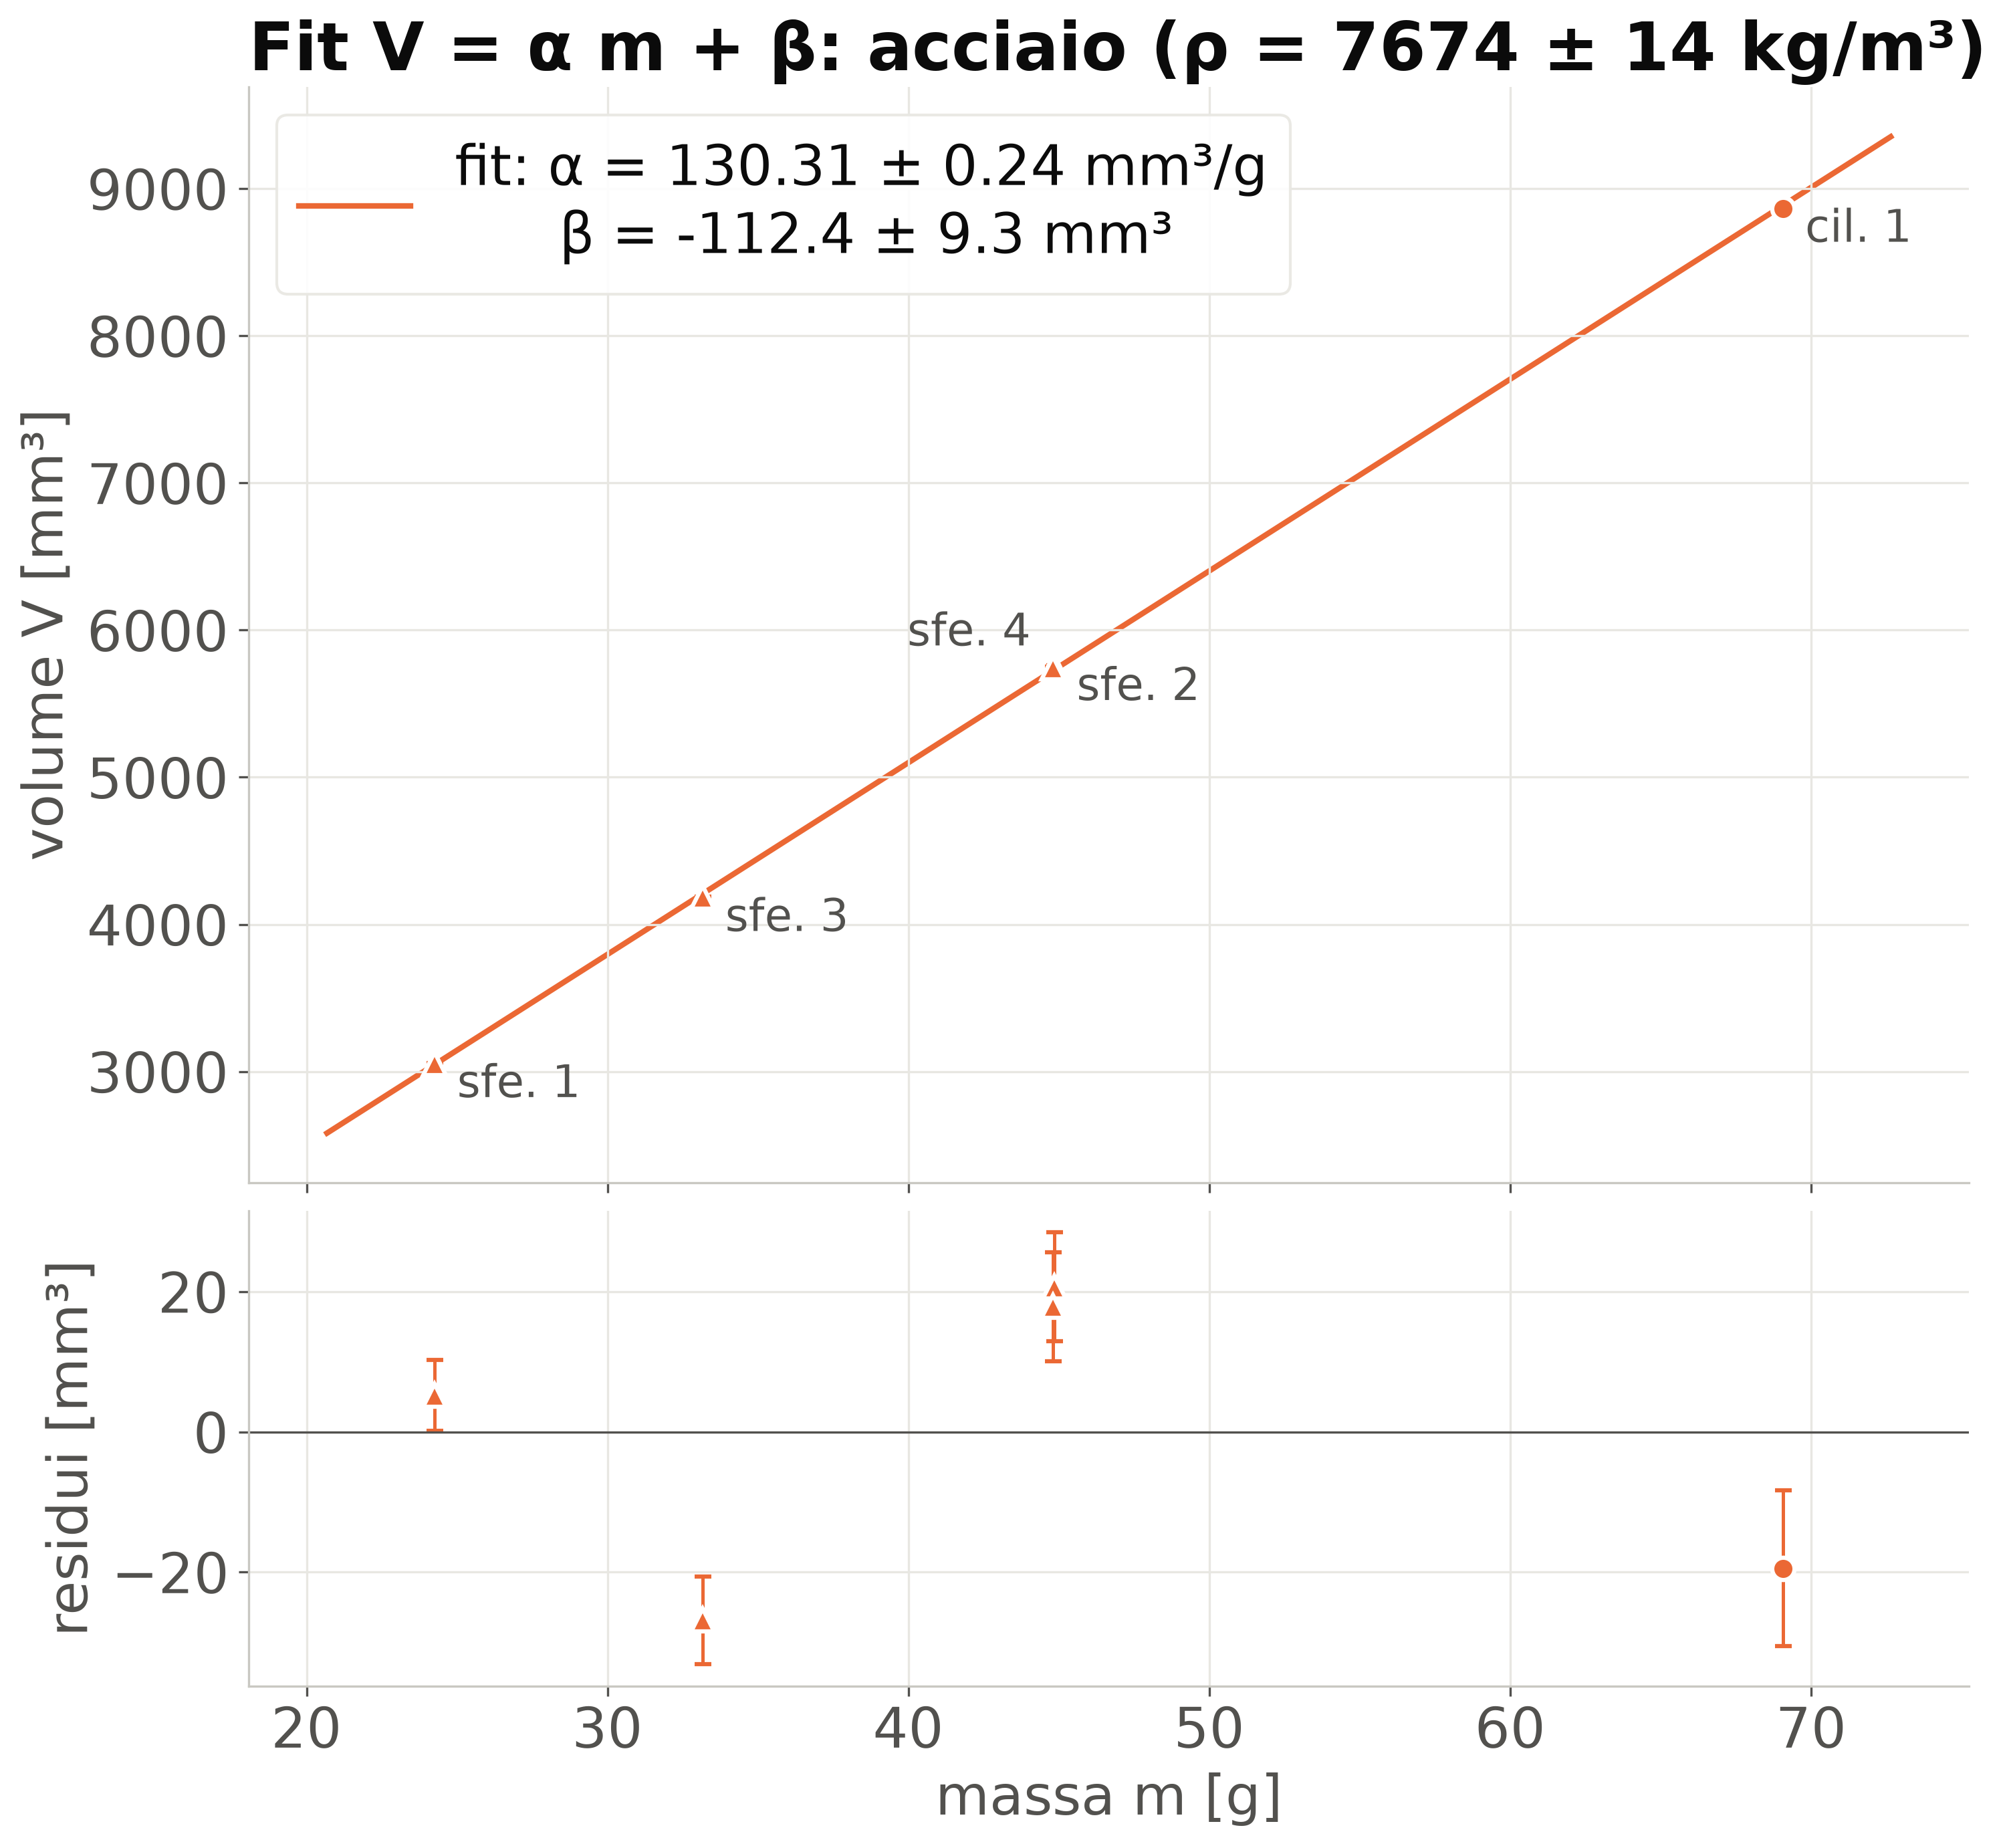
\includegraphics[width=0.62\linewidth]{grafici/b_fit_acciaio.png}
    \caption{Grafico di dispersione $(m,V)$, best fit per il primo gruppo di pesetti (acciaio) e grafico dei residui. I residui sono la differenza tra il volume misurato e quello previsto dalla retta, $r_i = V_i - (\alpha m_i + \beta)$, e mostrano quanto ogni punto sta sopra o sotto la retta. Se il fit \`e buono i residui sono sparsi intorno allo zero e distano da esso circa quanto la loro barra d'errore; qui invece alcuni punti (ad esempio la sfera 3) sono lontani dallo zero pi\`u di 4 barre d'errore.}
    \label{fig:densita1}
\end{figure}

\begin{figure}[htbp]
    \centering
     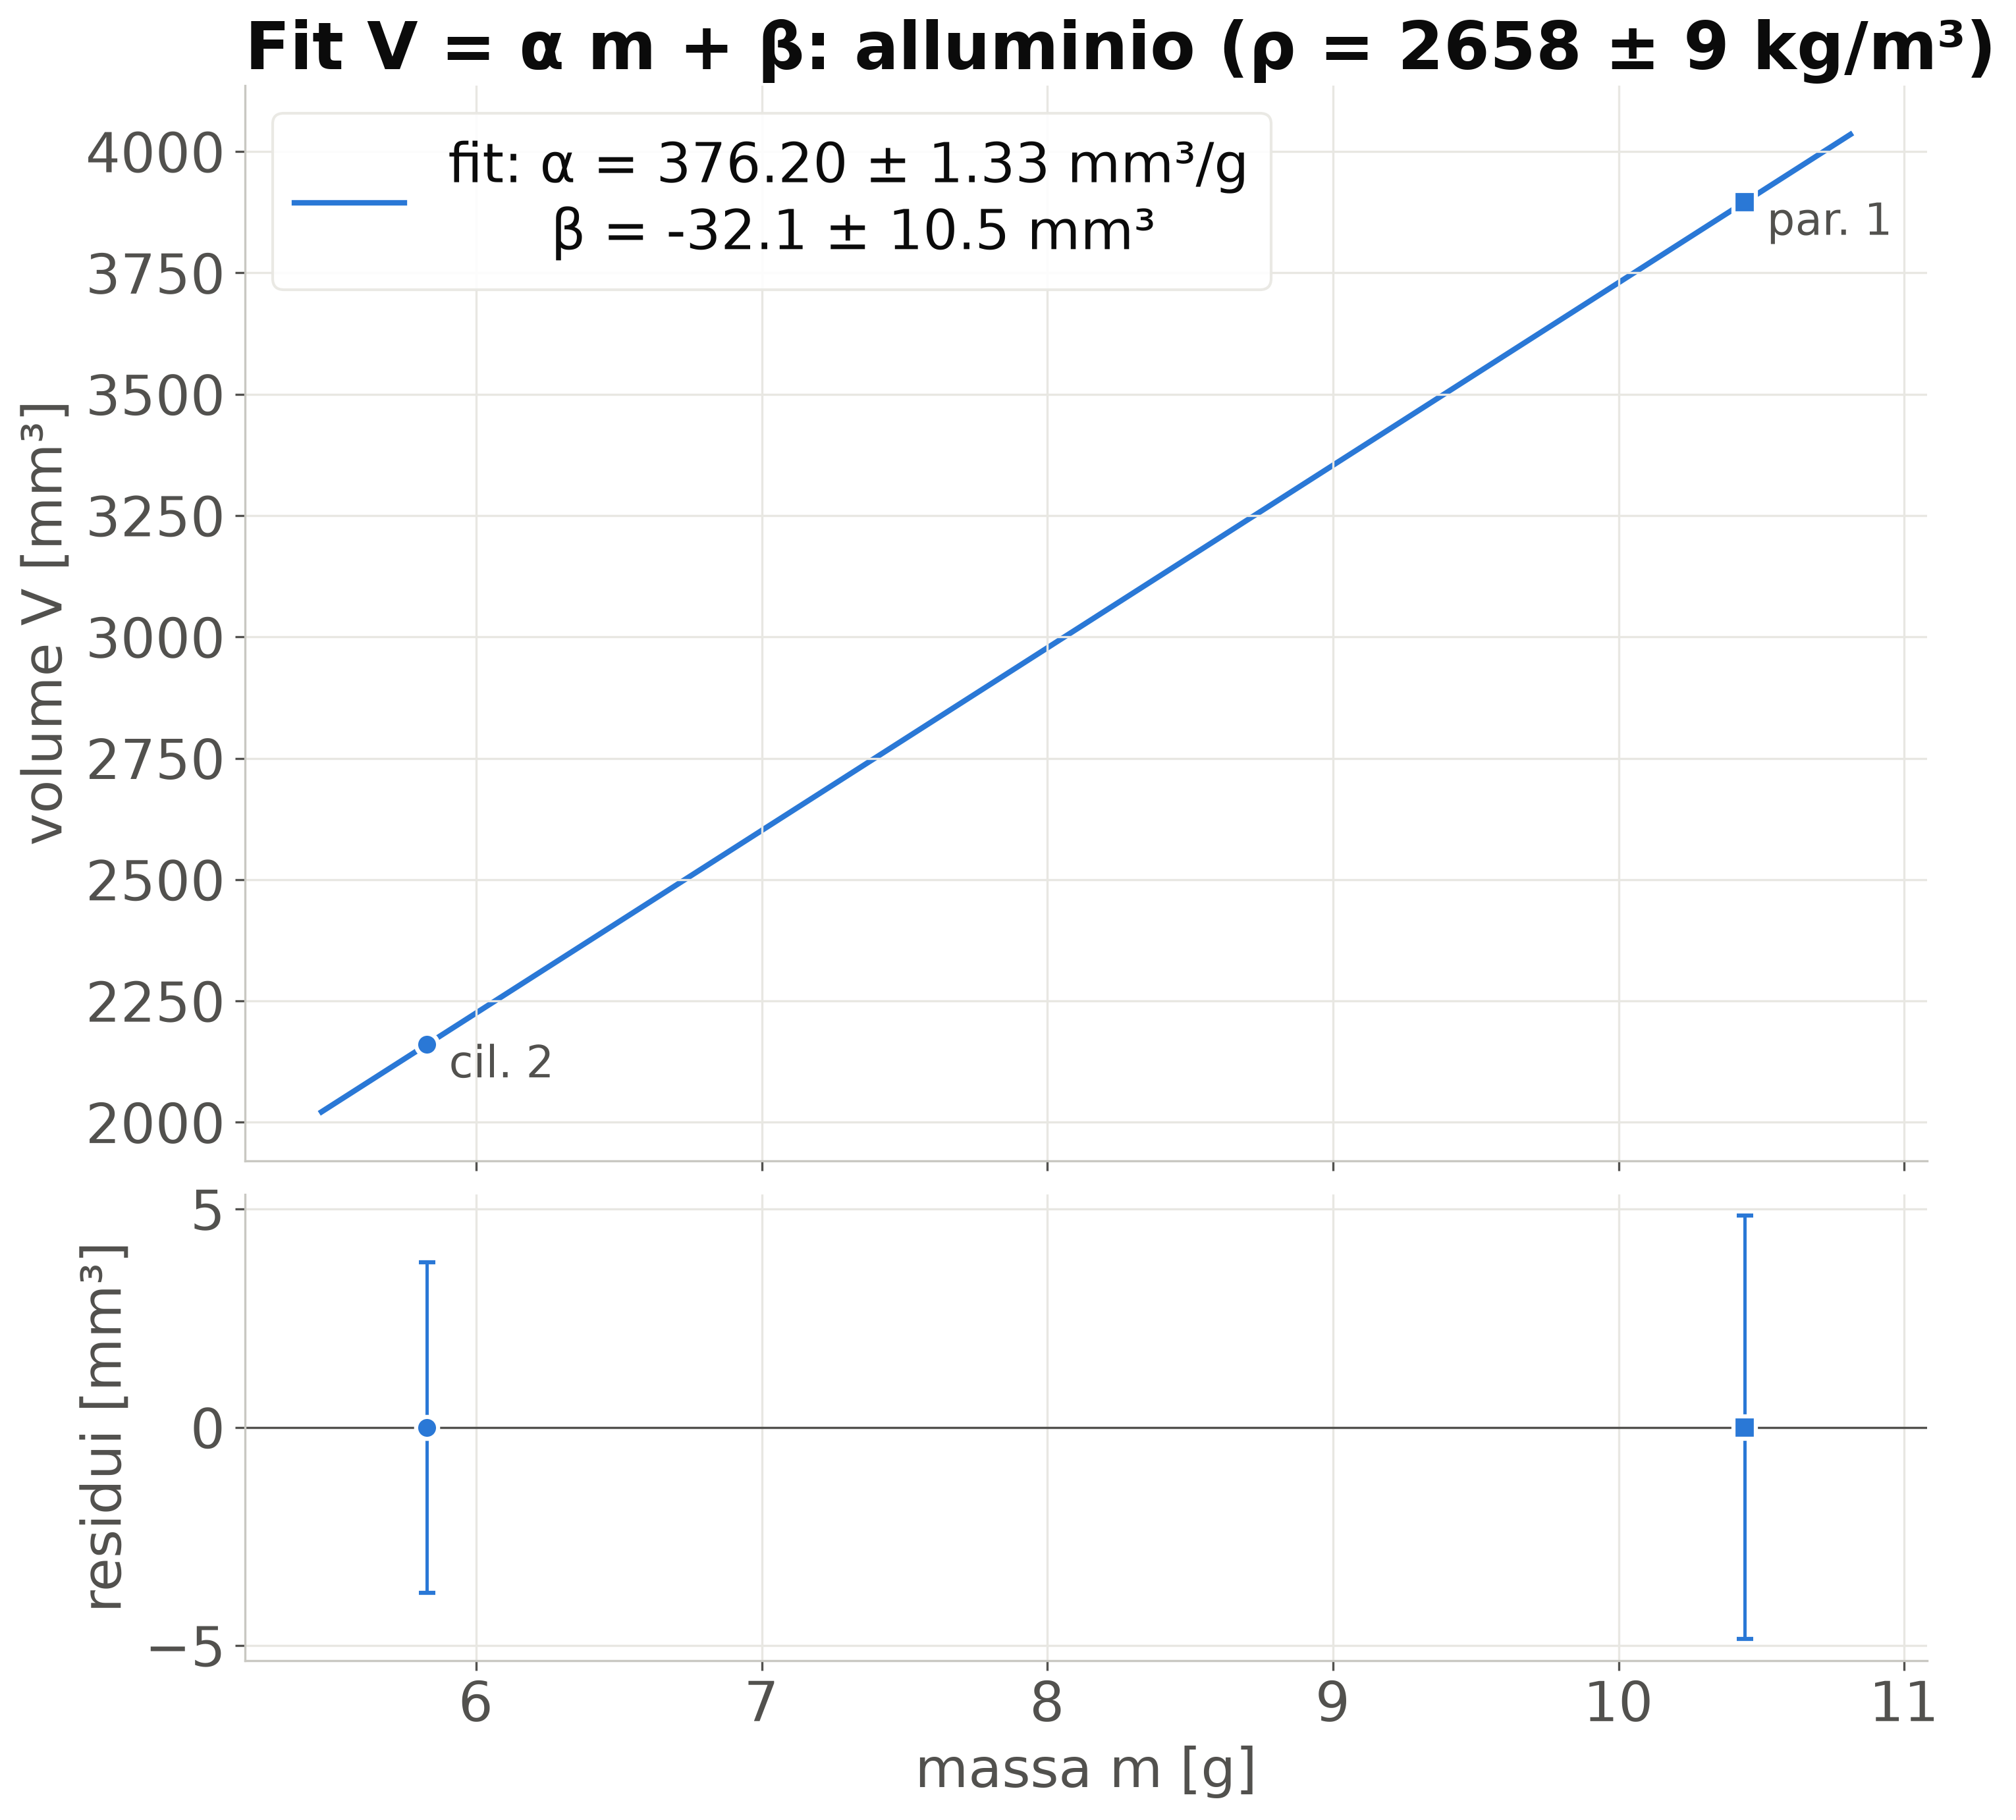
\includegraphics[width=0.62\linewidth]{grafici/b_fit_alluminio.png}
    \caption{Grafico di dispersione $(m,V)$, best fit per il secondo gruppo di pesetti (alluminio) e grafico dei residui (come in figura~\ref{fig:densita1}). I residui sono nulli perch\'e con due soli punti la retta passa esattamente per entrambi.}
    \label{fig:densita2}
\end{figure}

\begin{figure}[htbp]
    \centering
     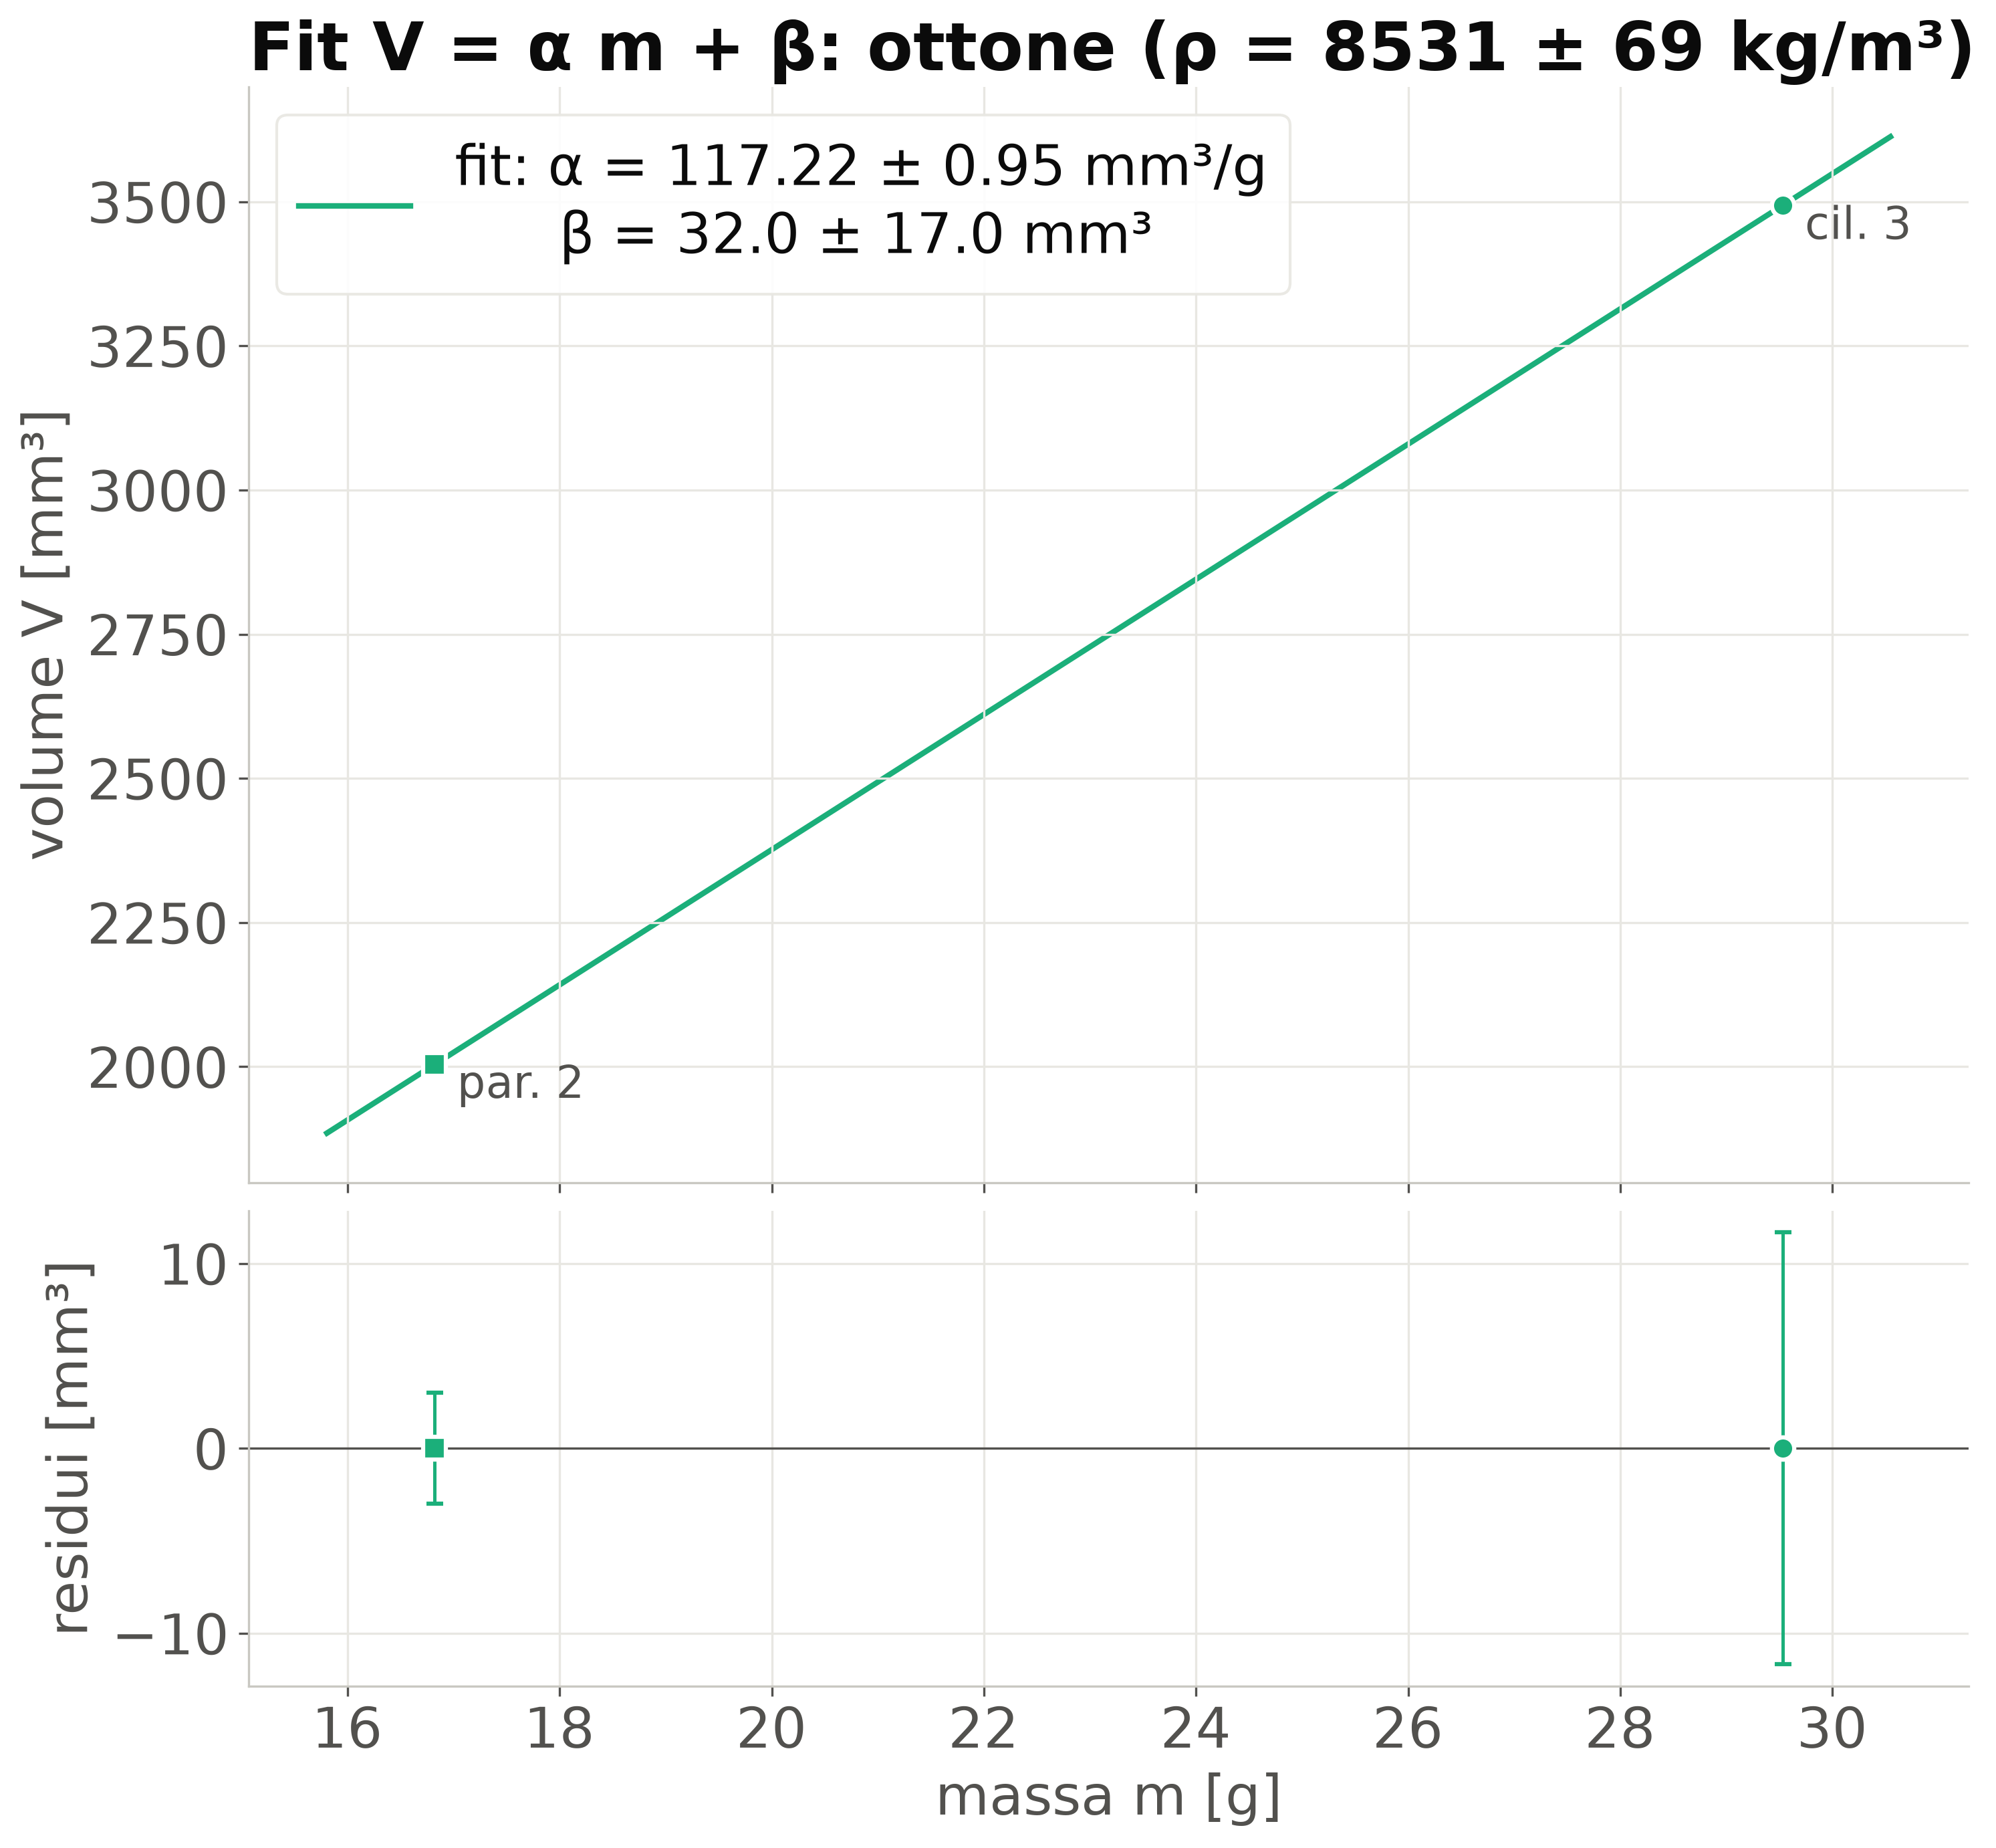
\includegraphics[width=0.62\linewidth]{grafici/b_fit_ottone.png}
    \caption{Grafico di dispersione $(m,V)$, best fit per il terzo gruppo di pesetti (ottone) e grafico dei residui (come in figura~\ref{fig:densita1}). Anche qui i punti sono due, quindi i residui sono nulli.}
    \label{fig:densita3}
\end{figure}

\begin{figure}[htbp]
    \centering
     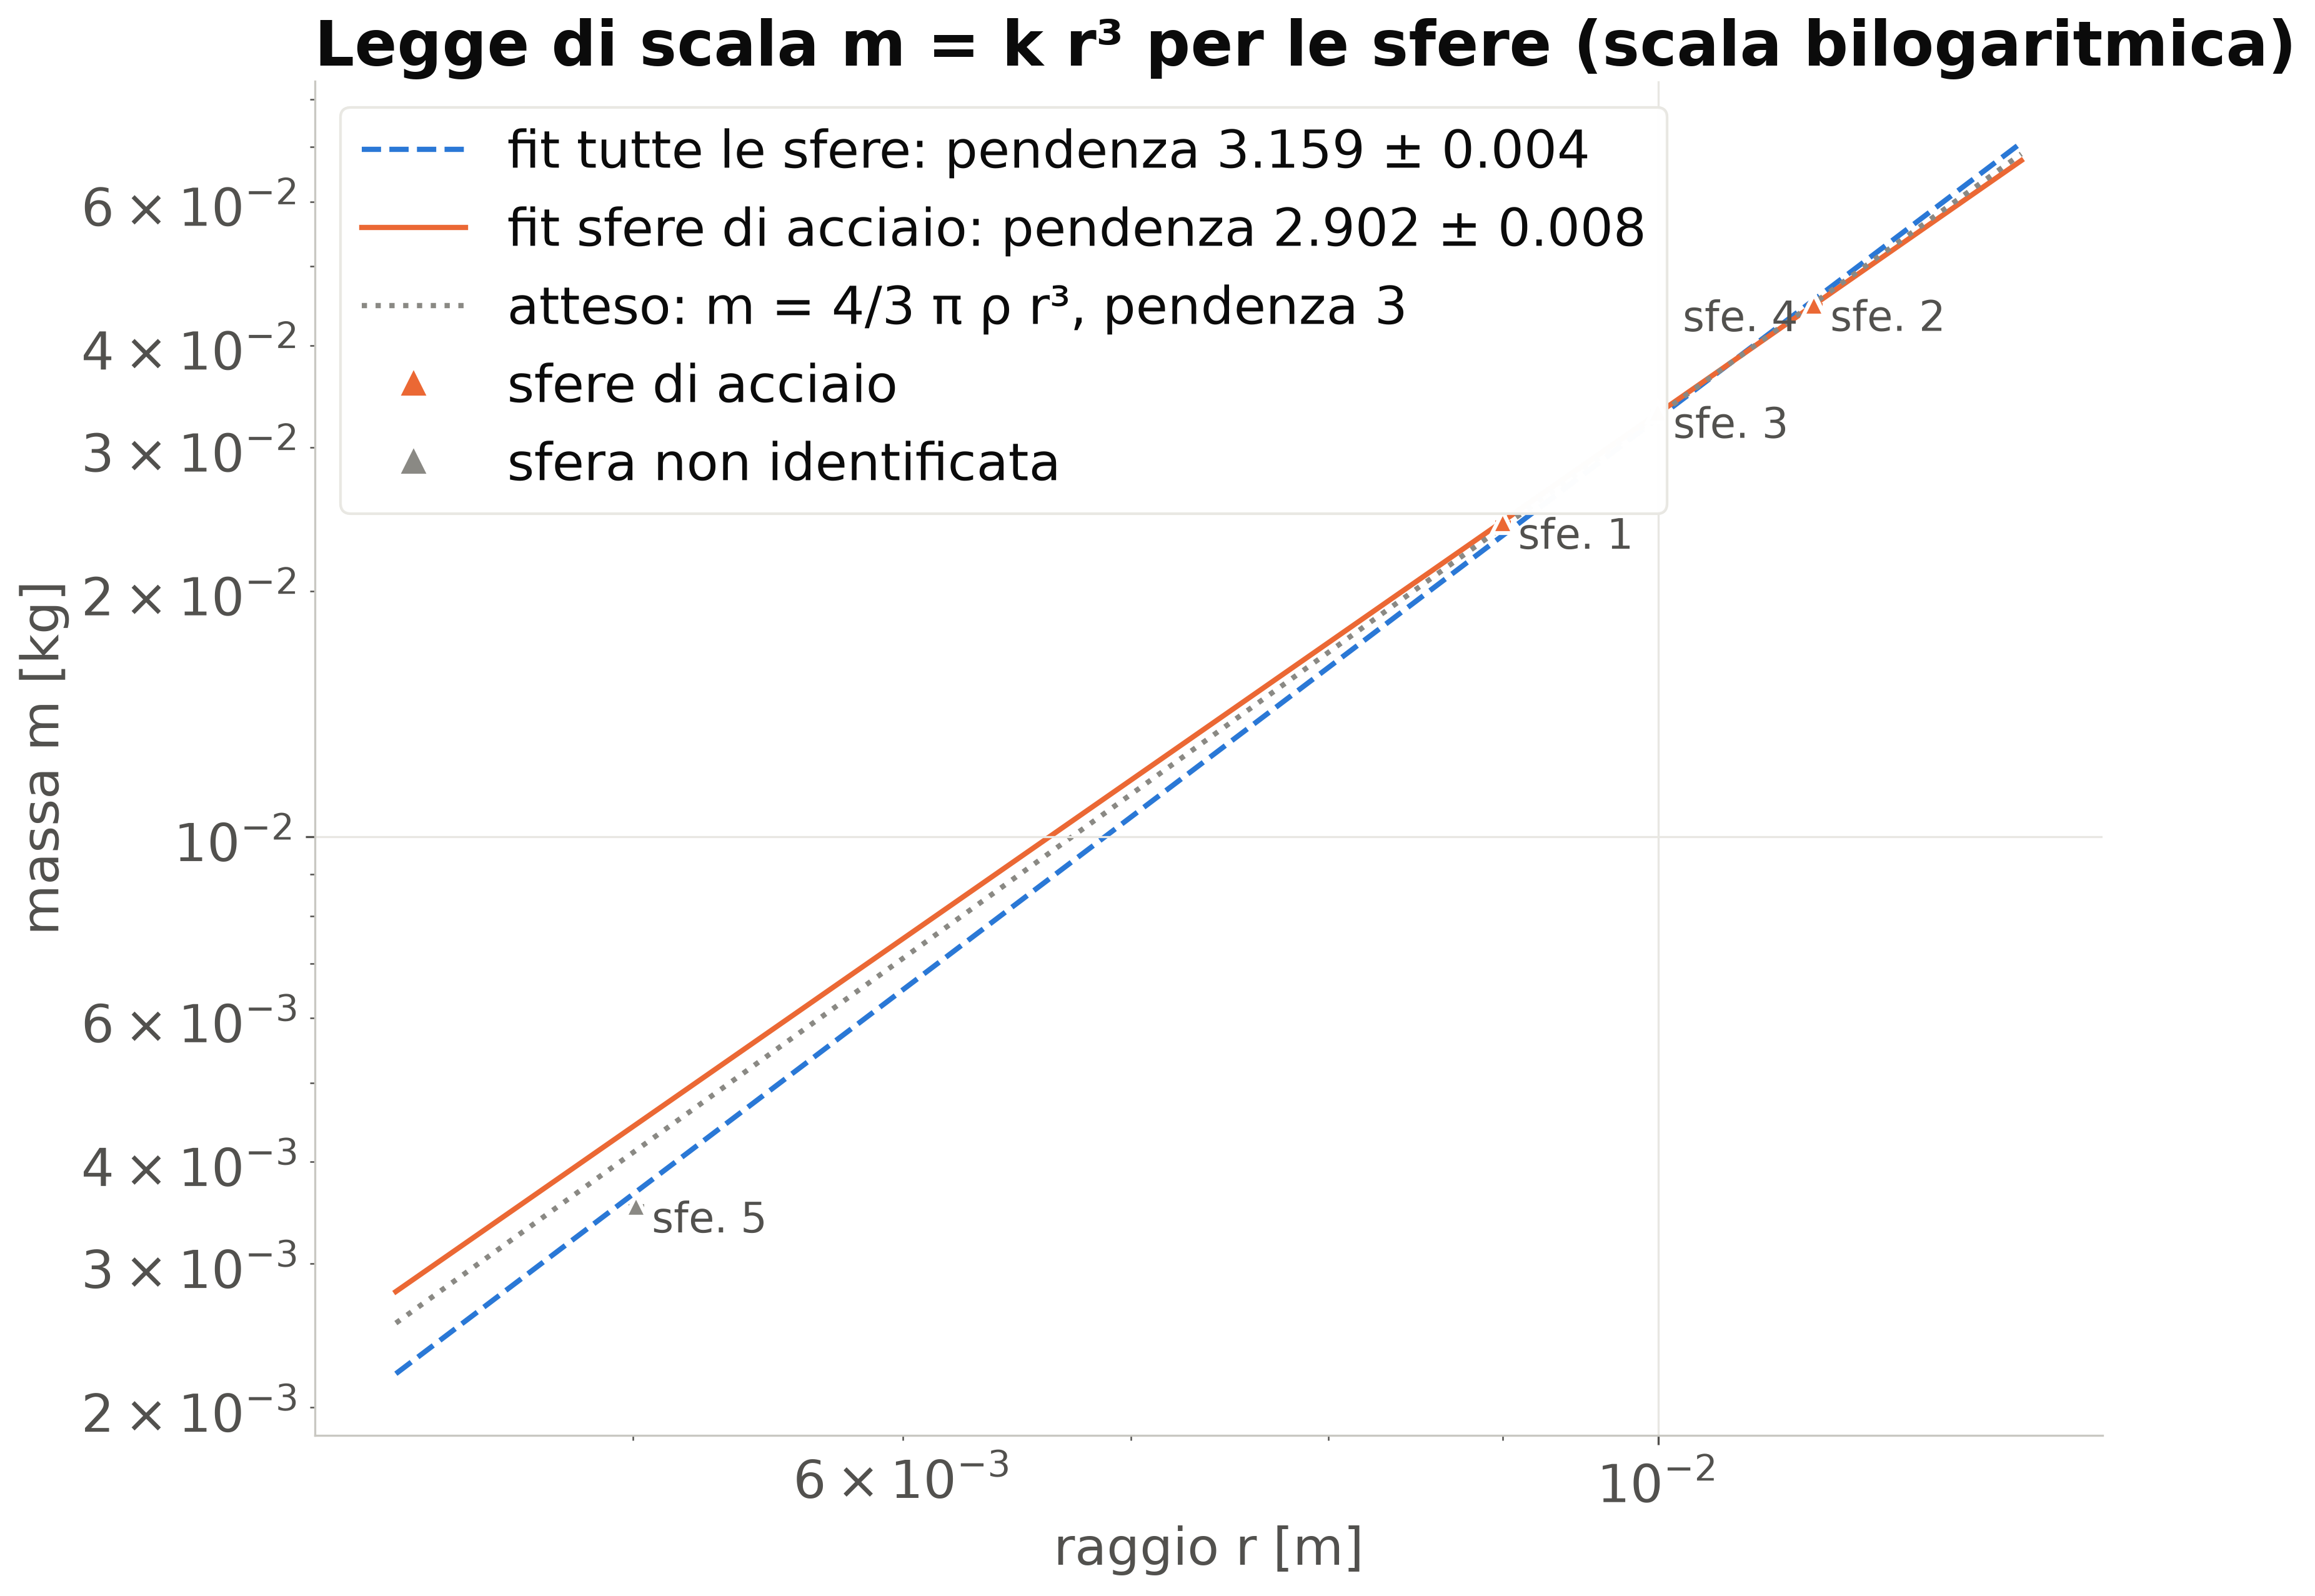
\includegraphics[width=0.75\linewidth]{grafici/7_legge_di_scala_sfere.png}
    \caption{Massa delle sfere in funzione del raggio in scala bilogaritmica, con i fit su tutte le sfere e sulle sole sfere di acciaio e la retta di pendenza 3 attesa.}
    \label{fig:legge_potenza}
\end{figure}